%===============================================================================
\section{Minimiza��o da norma $H_2$}
\label{sec:normH2}

Considerando o sistema apresentado em (\ref{eq:robust_sis_incert}) em malha fechada
com $\Delta \equiv 0$ e condi��o inicial nula. Um crit�rio normalmente utilizado 
� a norma $H_2$ da fun��o de transfer�ncia entre a entrada das perturba��es $\omega$
e a sa�da $z$. A norma $H_2$ pode ser calculada como em (\ref{eq:normh2_def}).

\begin{equation}
\left \| T(s) \right \|_2 \equiv \gamma _2=\sqrt{Tr(B_{\omega}'P_o B_{\omega})}
\label{eq:normh2_def}
\end{equation}

Onde :

\begin{equation}
P_o=\int_{0}^{\infty}((G-HK))e^{(A_0-BK)}B_{\omega})'((G-HK))e^{(A_0-BK)}B_{\omega})dt
\nonumber
\end{equation}

{\it{Interpreta��o estoc�stica da norma $H_2$}}: Se considerarmos $\omega(t)$ como sendo 
ruido branco, ent�o a norma $H_2$ de $T(s)$ � o valor da vari�ncia assint�tica da sa�da $z(t)$:

\begin{equation}
\left \| T(s) \right \|_2=\sqrt{\lim_{t\rightarrow \infty}E(z(t)'z(t))}
\nonumber
\end{equation}

{\it{Interpreta��o determin�stica da norma $H_2$}}: D� a ideia da energia da sa�da $z(t)$ 
em resposta as condi��es iniciais nulas.

\begin{equation}
\int_{0}^{\infty}z(t)'z(t)dt=x_0'P_o x_0
\nonumber
\end{equation}

Assim tendo que a norma pode ser apresentada como a seguir:

\begin{equation}
\left \| T(s) \right \|_2=\sqrt{\sum_{i=1}^{n_w} \int_{0}^{\infty}\left \| z^{i}(t) \right \|^2 dt}
\nonumber
\end{equation}

%===============================================================================
\subsection{Sistemas Lineares sem incertezas}
\label{sec:h2_sis_lin_sem_incertezas}

Se considerarmos o sistema (\ref{eq:robust_sis_incert}) com condi��es iniciais nulas e $\Delta \equiv 0$
temos o sistema apresentado em (\ref{eq:normh2_sis_sem_incertezas}).

\begin{equation}
\left\{\begin{matrix}
\dot{x}(t)=(A_0-B_0 K)x(t)+B_{\omega}\omega(t)
\\
z(t)=(G-HK)x(t)
\end{matrix}\right.
\label{eq:normh2_sis_sem_incertezas}
\end{equation}

Pode-se desta forma minimizar o escalar $\gamma_2$ sujeito a (\ref{eq:normh2_relim}).

\begin{equation}
\begin{matrix}
\gamma_2^2 > Tr(M)
\\ 
\\
\begin{bmatrix}
M & B_{\omega}'\\ 
B_{\omega} & W
\end{bmatrix} > 0
\\ 
\\ 
\begin{bmatrix}
-WA_0'+R'B_0'-A_0W +B_0R & (GW-HR)' \\ 
(GW-HR) & I
\end{bmatrix} >0
\end{matrix}
\label{eq:normh2_relim}
\end{equation}

%===============================================================================
\subsection{Incertezas do tipo polit�pico}
\label{sec:normh2_politopico}

Para um sistema com incertezas do tipo politopico ter garantia do limite superior de $\gamma_2$ 
para a norma $H_2$ de todos os sistemas pertencentes ao conjunto de sistemas formados pelas
incertezas � satisfeita para:

\begin{equation}
\begin{matrix}
\gamma_2^2 > Tr(M)
\\ 
\\
\begin{bmatrix}
M & B_{\omega}'\\ 
B_{\omega} & W
\end{bmatrix} > 0
\\ 
\\ 
\begin{bmatrix}
-WA_i'+R'B_j'-A_i W +B_j R & (GW-HR)' \\ 
(GW-HR) & I
\end{bmatrix} >0
\\
\forall i=1,...,na
\\
\forall j=1,...,nb
\end{matrix}
\nonumber
\end{equation}

%===============================================================================
\subsection{Incertezas limitadas em norma}
\label{sec:normh2_norm_limit}

Para o caso de incertezas com norma limitada temos (\ref{eq:normh2_norm_limit}).


\begin{equation}
\begin{matrix}
\gamma _2^2 > Tr(B_{\omega}'W^{-1}B_{\omega})
\\ 
\\
\begin{bmatrix}
Y & (E_AW-E_BR)' & (GW-HR)'\\ 
(E_AW-E_BR) & I & 0\\ 
 (GW-HR) & 0 & I
\end{bmatrix} \geq 0
\\ 
\\ 
Y=-WA_0'+R'B_0'-A_0W +B_0R -DD'
\end{matrix}
\label{eq:normh2_norm_limit}
\end{equation}

Com a realimenta��o $K=RW^{-1}$.
%===============================================================================
\subsubsection{Simula��o}

A resolu��o do sistema de LMIs (\ref{eq:normh2_norm_limit}) gerou os seguintes resultados:

\begin{equation}
\begin{matrix}
W=\begin{bmatrix}
0.4644 &  -0.0305\\
-0.0305 &   0.7975
\end{bmatrix}\\ \\ 
R=1.10^3\begin{bmatrix}
0.0009 &  -8.6987
\end{bmatrix}
\\ \\
K=1.10^4\begin{bmatrix}
-0.0716 &  -1.0935
\end{bmatrix}
\\ \\
M =  0.0170
\\
\lambda_1=-0.0326\\
\lambda_2=-1.7666
\end{matrix}
\nonumber
\end{equation}

A simula��o do sistema em malha fechada com o ganho $K$ encontrado obtem a resposta
apresentada na Figura (\ref{fig:h2_norm_bounded}). Os valores de $\lambda_1$ e $\lambda_2$ 
s�o os autovalores do sistema em malha fechada.

\begin{figure}[htbp]
	\center
	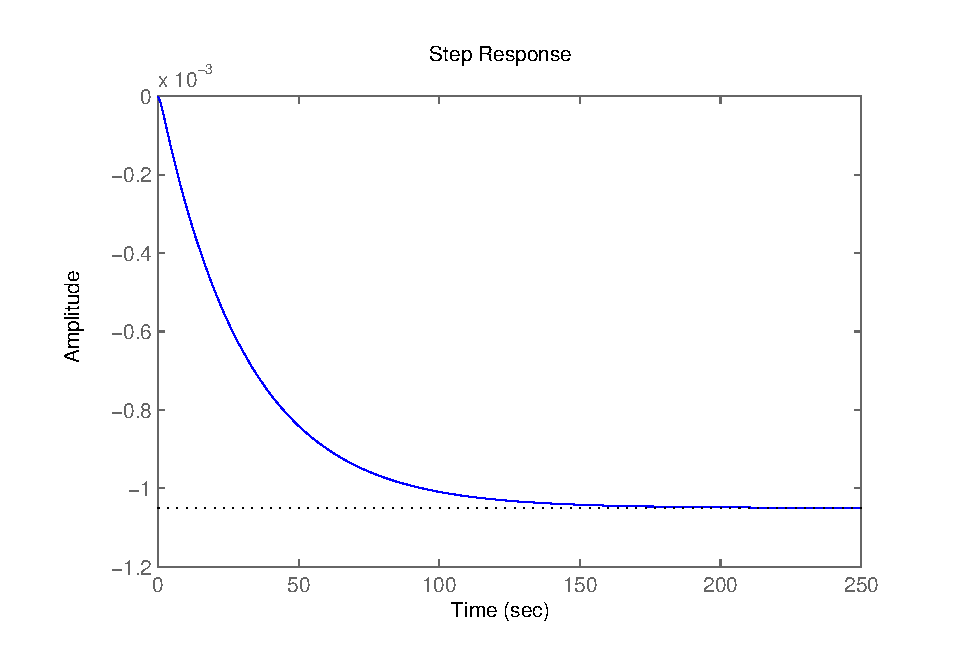
\includegraphics[width=0.95\columnwidth]{figures/h2_norm_bounded.eps}
	\caption{Resposta do sistema (\ref{eq:sis_mf_incerteza}) com o ganho K encontrado 
		pelo crit�rio de $H_2$}
	\label{fig:h2_norm_bounded}
\end{figure}
